\documentclass{report}
\usepackage{graphicx}
\usepackage{multirow}
\usepackage{a4wide}
\usepackage{fancyhdr}
\usepackage{amsfonts}
\usepackage{amsmath}
\usepackage{subcaption}
\usepackage{color}
\setlength{\headheight}{15.2pt}
\pagestyle{fancy}
\newcommand{\docTitle}{Multibunch feedback application software}
\newcommand{\docAuthor}{A.~F.~D.~Morgan}
\newcommand\abs[1]{\left|#1\right|}
\rhead{\docTitle}
\rfoot{\docAuthor}
\lhead{}
\begin{document}
\title{
\begin{tabular}{|c|}
\hline
%\includegraphics[scale=0.5]{diamondlogo.png}\\
\hline
\large{\bf{\docTitle}}\\
\hline
\end{tabular}}
\author{\docAuthor}
\maketitle
\tableofcontents

\chapter{Overview}
The hardware for multi bunch feedback has many different possible settings.  Broadly speaking feedback system has a frontend which takes in the signals from the pickups, and does the initial analogue signal conditioning, connected to digital systems for each of the three planes (x,y,s). These digital systems calculate the feedback required and send signals to analogue drive electronics in order to excite the beam in the given plane.

\begin{figure}[hbt]
\begin{center}
  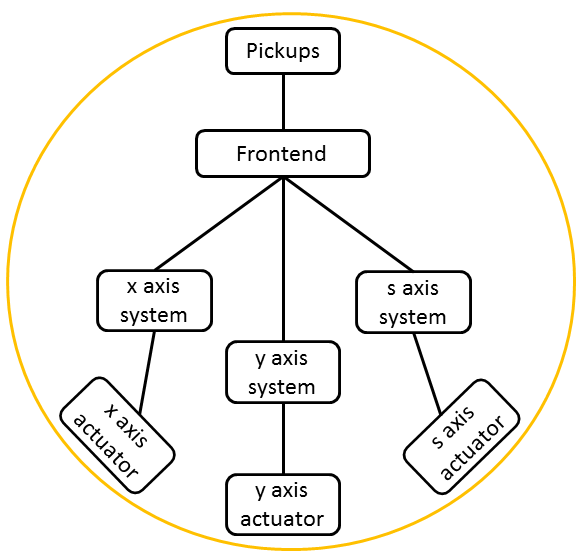
\includegraphics[width=0.5\textwidth]{top_level_system_overview.png}\\
  \caption{System overview}\label{system_overview}
\end{center}
\end{figure}

In order to make such a system more generally useable, this suite of task specific applications has been developed. All these codes save the relevant data and graphs to a file structure based on the date, and given unique names based on the date and time the application was run. The root path for this structure is defined in \verb|mbf_system_config.m|, as is the harmonic number of the machine under study. In general all machine/deployment parameters are set in this file. The rest of the codebase it written to adapt to what is set here.

Additional to the data from the multi bunch hardware, more general machine parameters are also captured for growdamp, modescan and bunch motion codes, in order to enable machine studies (e.g current dependance). This additional data is set in \verb|machine_environment.m|.


\chapter{Frontend phase scans}
In order to work optimally the feedback systems need to be matched in timing/phase with the beam phase (not the RF phase). Conceptually this comprises a master phase shifter (LO) which moves all three systems and allows the complete system to be adjusted to changes in beam phase, combined with three subsidiary phase shifters, one for each axis to allow the axes to be individually tuned.
\begin{figure}[hbt]
   \centering
    \begin{subfigure}[b]{0.45\textwidth}
        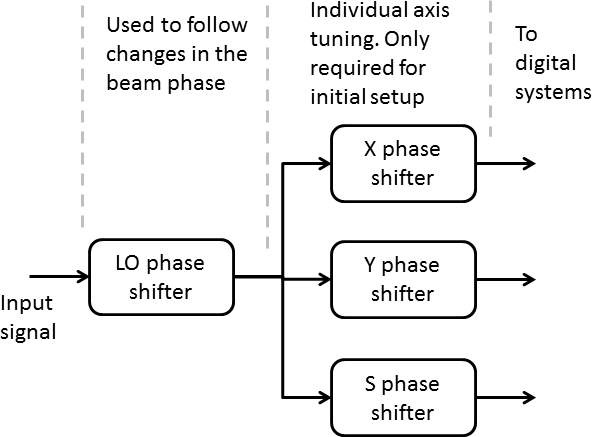
\includegraphics[width=\textwidth]{phase_shifters_overview.png}
        \caption{phase shifters}
        \label{fig:phase_shifters}
    \end{subfigure}
    ~ %add desired spacing between images, e. g. ~, \quad, \qquad, \hfill etc.
      %(or a blank line to force the subfigure onto a new line)
    \begin{subfigure}[b]{0.3\textwidth}
        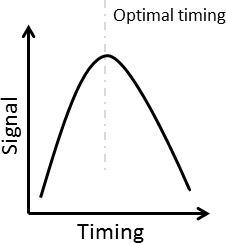
\includegraphics[width=\textwidth]{timing_overview.png}
        \caption{Clock timing}
        \label{fig:clock_timing}
    \end{subfigure}
    \caption{Conceptual diagrams}\label{fig:Conceptual_diagrams}
\end{figure}
Additionally, the timing of the clocks in the digital part of the system need to be tuned so that the sampling point coincides with the maximum signal from each bunch. This both increases the sampled signal, but also minimises the leakage to adjacent bunches.

\begin{figure}[hbt]
   \centering
    \begin{subfigure}[b]{0.3\textwidth}
        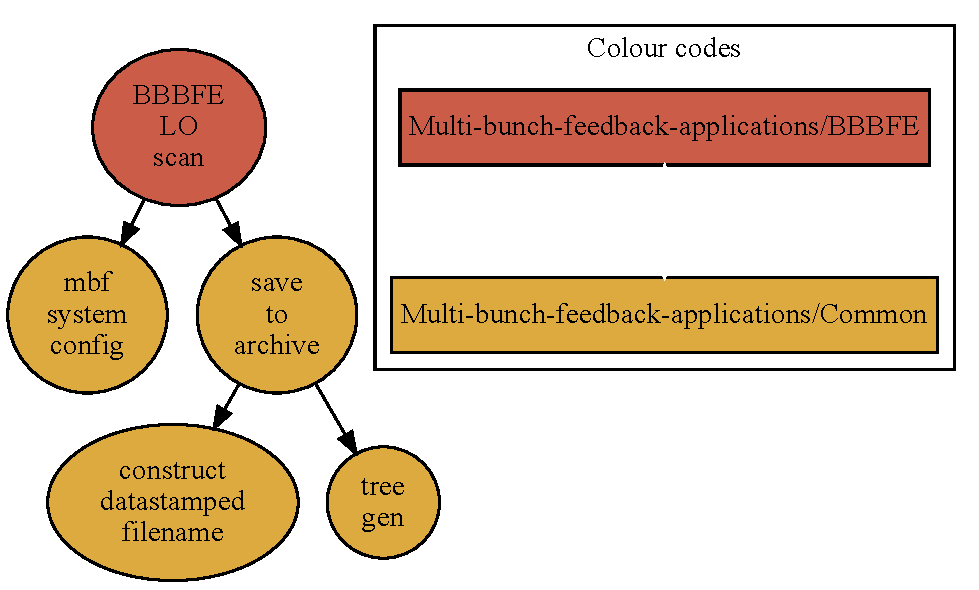
\includegraphics[width=\textwidth]{BBBFE_LO_scan.pdf}
        \caption{LO scan}
        \label{fig:LO_scan}
    \end{subfigure}
    ~ %add desired spacing between images, e. g. ~, \quad, \qquad, \hfill etc.
      %(or a blank line to force the subfigure onto a new line)
    \begin{subfigure}[b]{0.3\textwidth}
        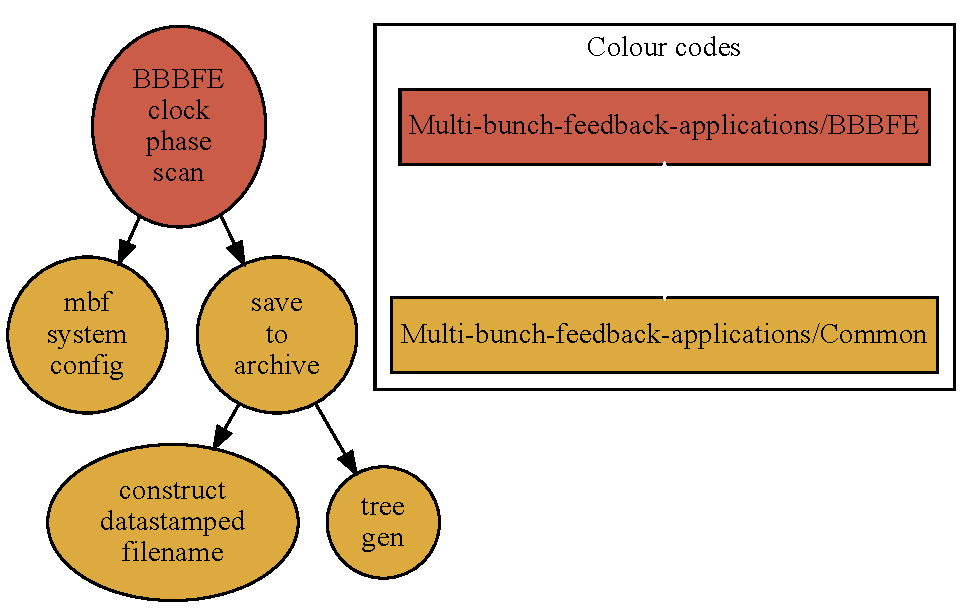
\includegraphics[width=\textwidth]{BBBFE_clock_phase_scan.pdf}
        \caption{Clock phase scan}
        \label{fig:clock_phase_scan}
    \end{subfigure}
    ~ %add desired spacing between images, e. g. ~, \quad, \qquad, \hfill etc.
    %(or a blank line to force the subfigure onto a new line)
    \begin{subfigure}[b]{0.3\textwidth}
        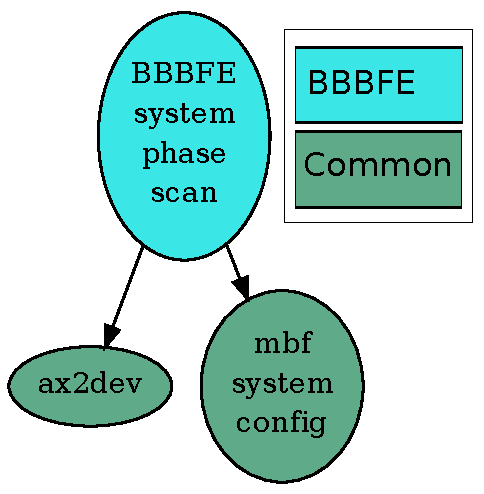
\includegraphics[width=\textwidth]{BBBFE_system_phase_scan.pdf}
        \caption{System phase scan}
        \label{fig:system_phase_scan}
    \end{subfigure}
    \caption{Code trees for bunch by bunch frontend scans}\label{fig:BBBFE_code_trees}
\end{figure}

Typical output:

Often you can just use \verb|BBBFE_LO_scan| to tune all four phase shifters, as one is aiming to have the peaks of the three curves at the same phase angle.

\section{Examples}

Scan the local oscillator 45 degrees either side of 90 degrees. This is the first check to see if the three systems are aligned to the beam phase.
\begin{verbatim}
BBBFE_LO_scan(90, 45)
\end{verbatim}

The next two examples are done on an individual axis at a time. \textcolor{red}{Sort out the mapping of clocks to axes.}
\begin{verbatim}
Setup: (manual for the time being...)
press tune only
fill some charge in bunch 1 (0.2nC)
set bunch mode single bunch
set single bunch 1
press setup tune
set up individual tune detectors to run on the selected bunch and one bunch either side.
set sweep gain to -18
set detector fixed gain
\end{verbatim}
\begin{verbatim}
BBBFE_clock_phase_scan(1)
\end{verbatim}
\begin{verbatim}
BBBFE_system_phase_scan('X')
\end{verbatim}
\chapter{Mode scans}

%\begin{figure}[hbt]
%\begin{center}
%  \includegraphics[width=0.5\textwidth]{mbf_modescan_top_level.pdf}\\
%  \caption{System overview}\label{fig:code_tree_modescan}
%\end{center}
%\end{figure}

\section{Examples}

\begin{verbatim}
mbf_modescan_top_level('x')
\end{verbatim}


\chapter{Spectra}
This code captures the requested number of turns from the requested axis and returns the FFT of the centroid motion of each bunch.

\begin{figure}[hbt]
\begin{center}
  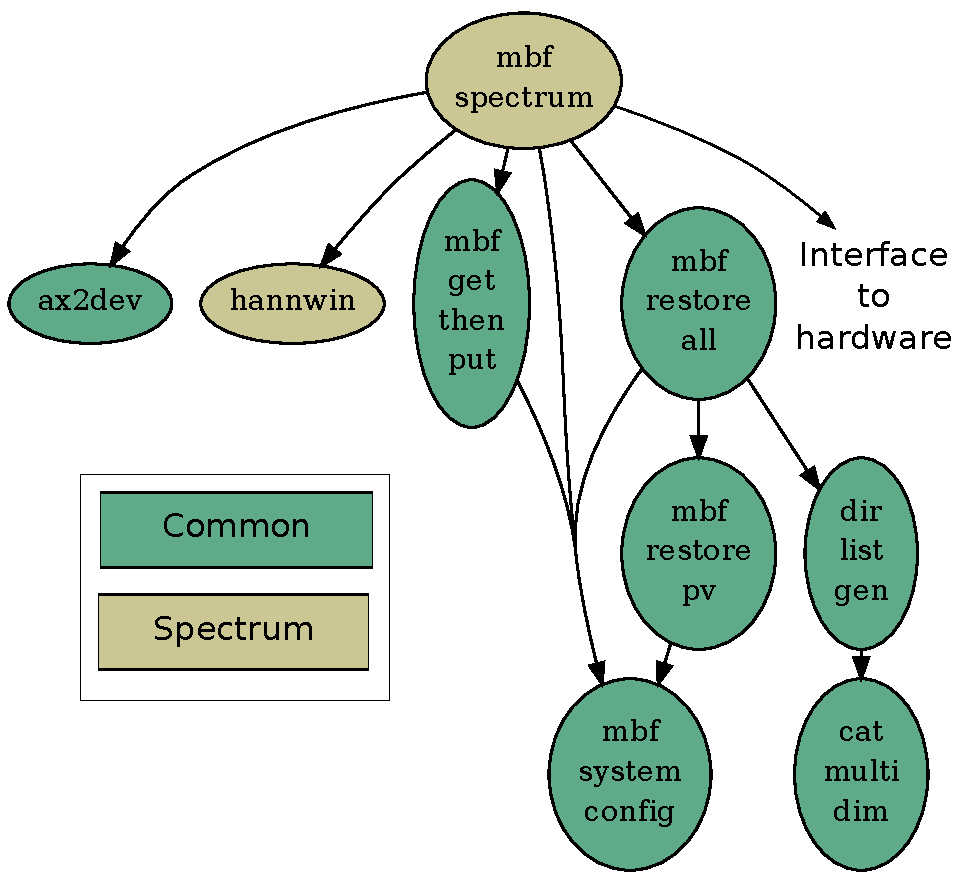
\includegraphics[width=0.5\textwidth]{mbf_spectrum.pdf}\\
  \caption{System overview}\label{fig:code_tree_spectrum}
\end{center}
\end{figure}

Typical output:


\section{Examples}

\begin{verbatim}
[f_magnitude,f_phase] = mbf_spectrum('x', 100)
\end{verbatim}

\chapter{Growdamp}
The measurement comprises a series of excitations at set frequencies followed by capture of the evolution of bunch centroid positions.
\section{Capturing data}
The parameters for the length of excitation and  capture are set in \verb|mbf_growdamp_config.m|. The \verb|mbf_growdamp_setup| code sets up the hardware for the correct type of measurement. \verb|mbf_growdamp_capture| triggers the measurement, captures the data and stores it in the file structure defined in \verb|mbf_system_config|. Finally \verb|mbf_restore_all| returns the settings for the MBF system to their original states.

\begin{figure}[hbt]
   \centering
    \begin{subfigure}[b]{0.45\textwidth}
        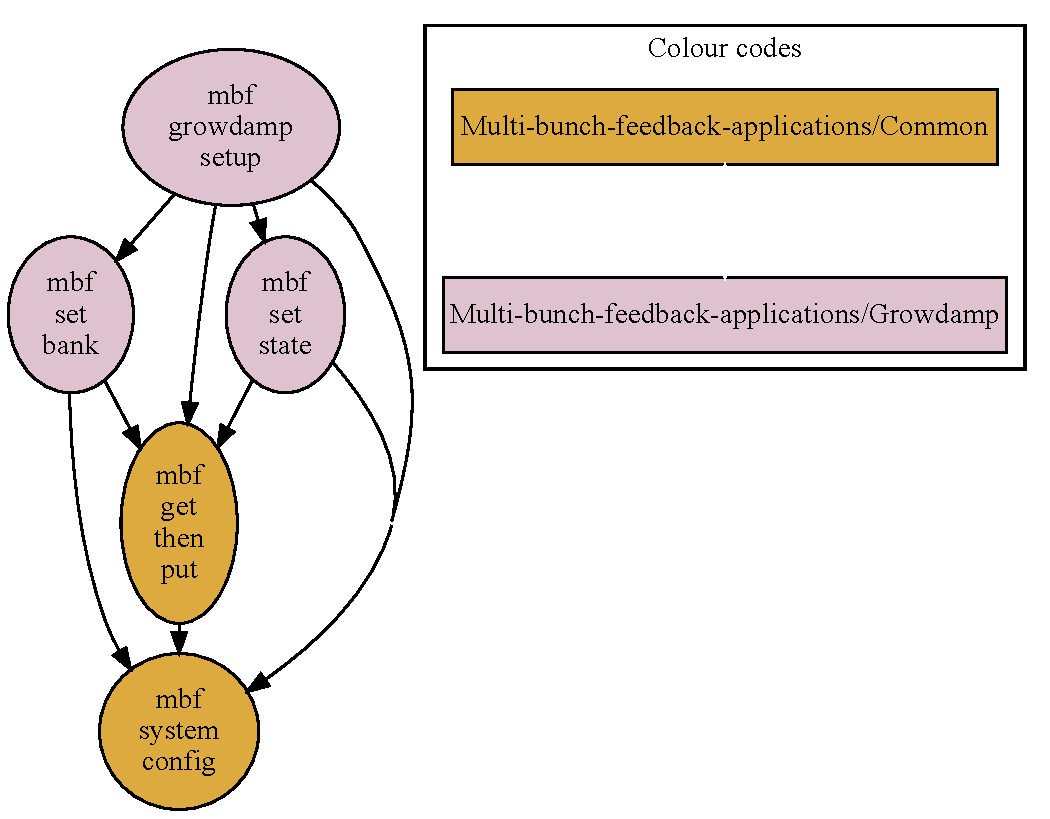
\includegraphics[width=\textwidth]{mbf_growdamp_setup.pdf}
        \caption{Sets up the system for a grow damp measurement}
        \label{fig:growdamp_setup}
    \end{subfigure}
    ~ %add desired spacing between images, e. g. ~, \quad, \qquad, \hfill etc.
      %(or a blank line to force the subfigure onto a new line)
    \begin{subfigure}[b]{0.45\textwidth}
        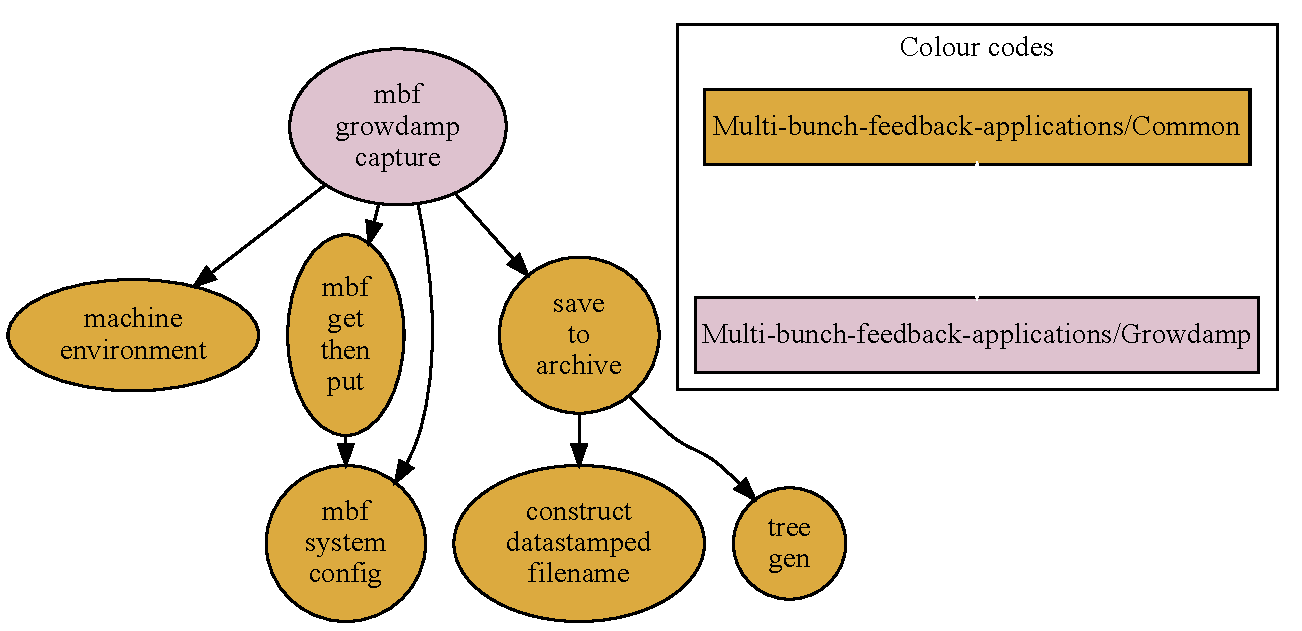
\includegraphics[width=\textwidth]{mbf_growdamp_capture.pdf}
        \caption{Captures grow damp data}
        \label{fig:growdamp_capture}
    \end{subfigure}
    \caption{Code trees to run a grow damp experiment}\label{fig:growdamp_code_trees1}
\end{figure}

\begin{figure}[hbt]
   \centering
    \begin{subfigure}[b]{0.3\textwidth}
        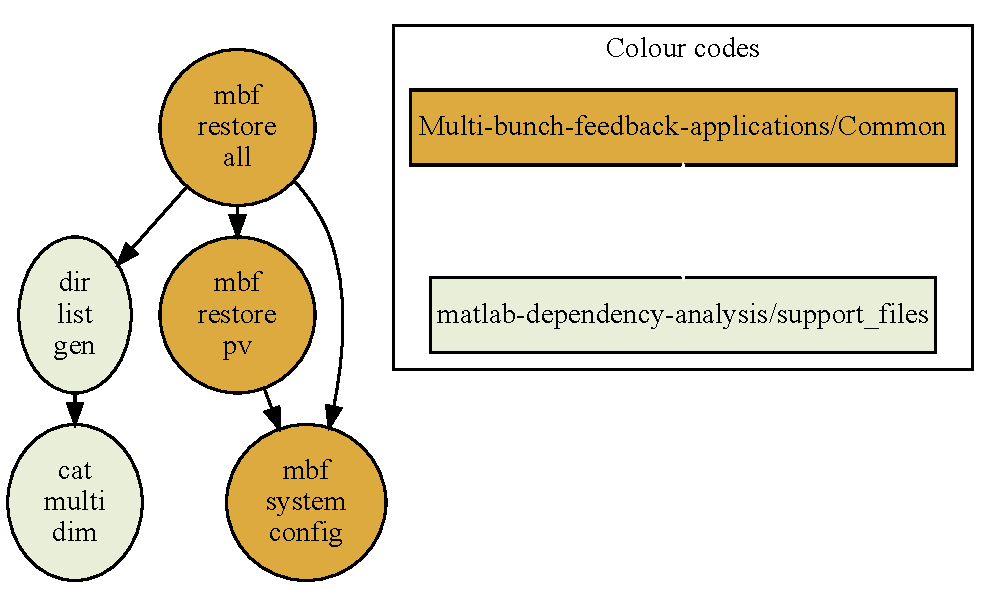
\includegraphics[width=\textwidth]{mbf_restore_all.pdf}
        \caption{Restore the mbf system }
        \label{fig:restore}
    \end{subfigure}
        \begin{subfigure}[b]{0.3\textwidth}
        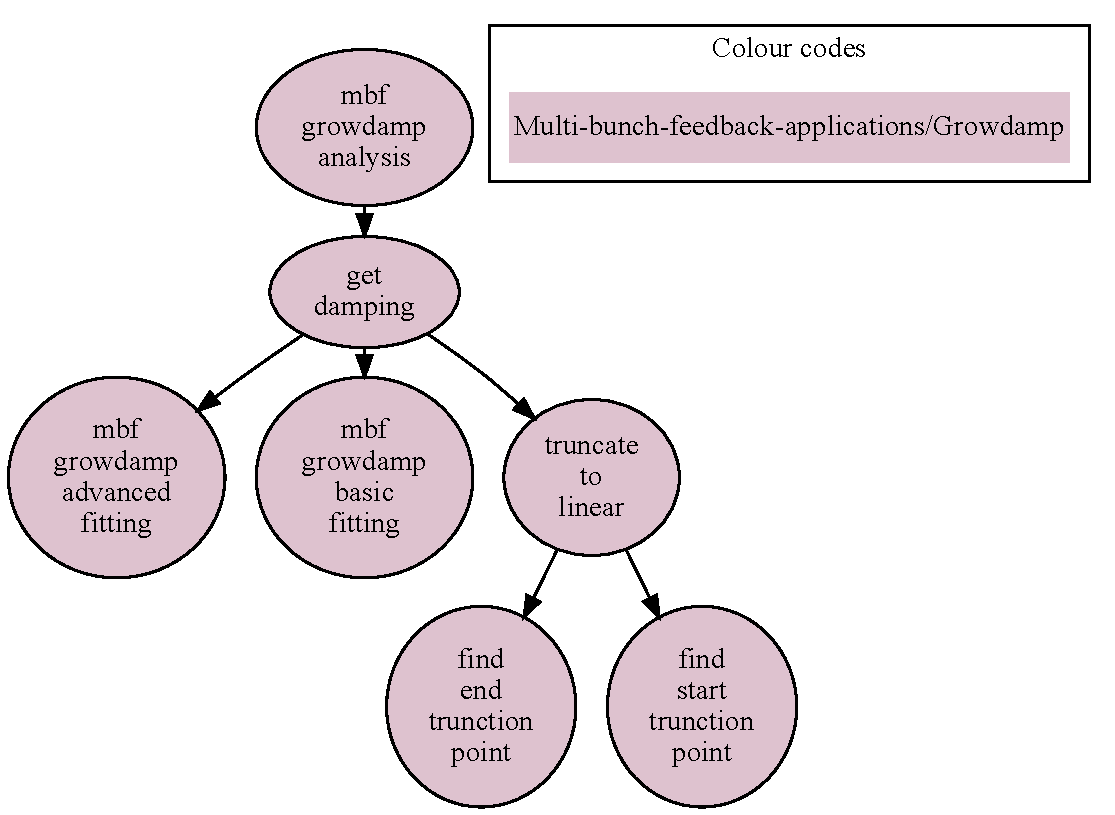
\includegraphics[width=\textwidth]{mbf_growdamp_analysis.pdf}
        \caption{For analysing a data set}
        \label{fig:growdamp_analysis}
    \end{subfigure}
    \caption{Code trees to restore the mbf system and analyse the data}\label{fig:growdamp_code_trees2}
\end{figure}

\section{Analysing saved data}
Although one can analyse the data imediately using \verb|mbf_growdamp_analysis|, it is often more useful to analyse a set of previously captured data. \verb|mbf_growdamp_archival_retrival| will return all the data sets within a user defined time period. These data sets can then be passed to \verb|mbf_growdamp_archival_analysis| where the data can either just be plotted for visual comparison, be averaged, or to be plotted against one of the machine parameters also stored in the data sets.

\begin{figure}[hbt]
   \centering
    \begin{subfigure}[b]{0.3\textwidth}
        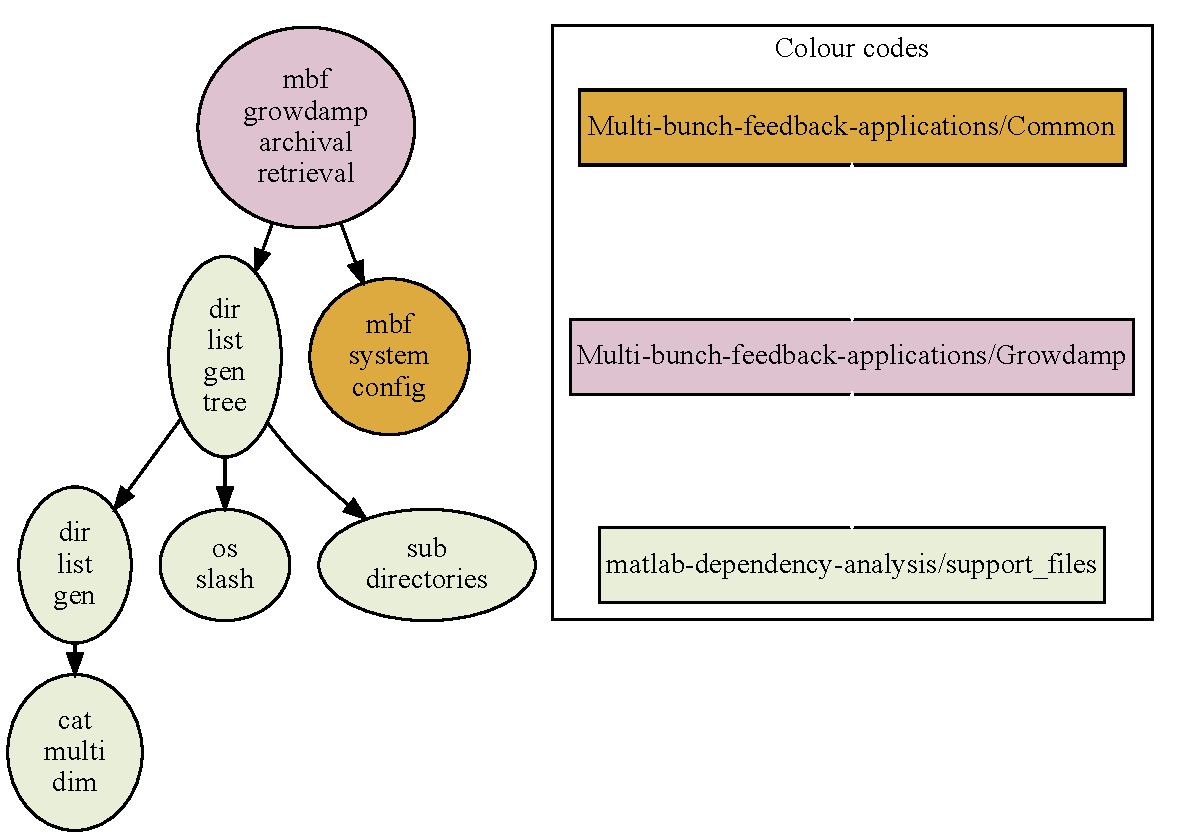
\includegraphics[width=\textwidth]{mbf_growdamp_archival_retrieval.pdf}
        \caption{For retriving data sets from the data store}
        \label{fig:growdamp_archiving_retrival}
    \end{subfigure}
    ~ %add desired spacing between images, e. g. ~, \quad, \qquad, \hfill etc.
      %(or a blank line to force the subfigure onto a new line)
    \begin{subfigure}[b]{0.3\textwidth}
        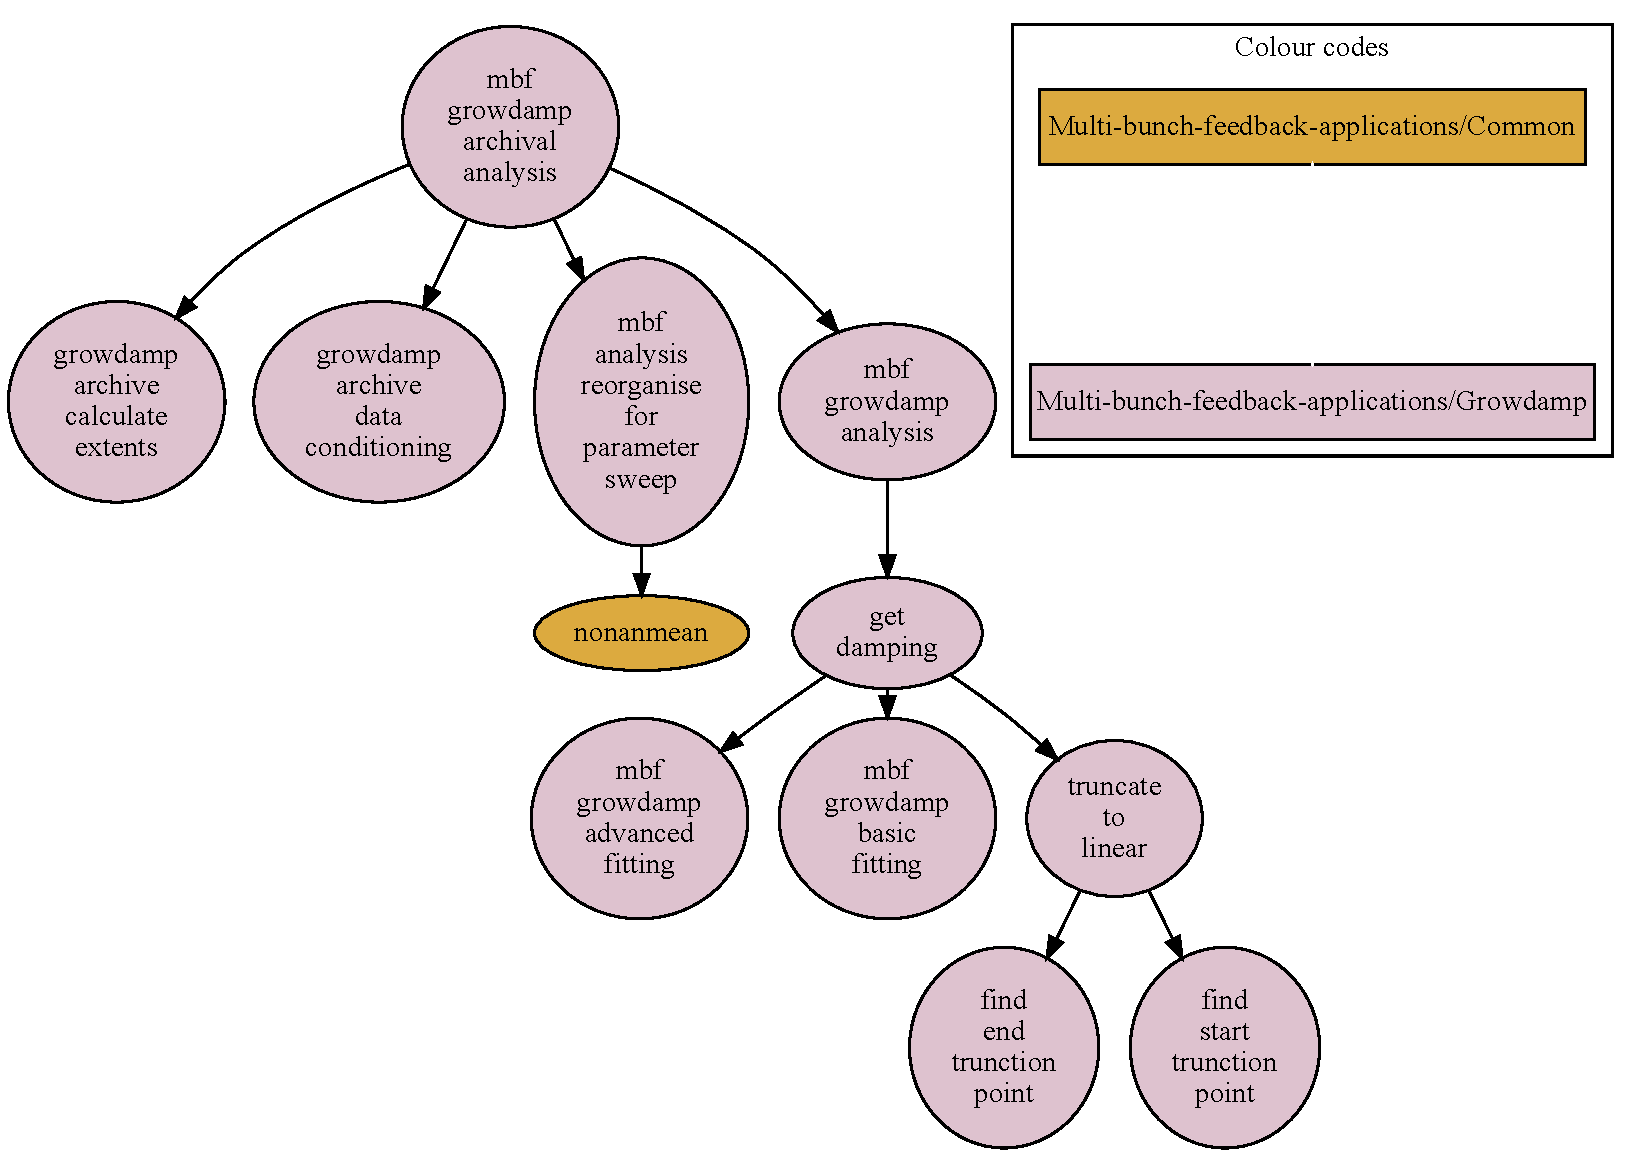
\includegraphics[width=\textwidth]{mbf_growdamp_archival_analysis.pdf}
        \caption{For analysing data sets (display, averaging, parameter scans)}
        \label{fig:growdamp_archiving_analysis}
    \end{subfigure}
    \caption{Code trees grow damp archival analysis}\label{fig:growdamp_archival_code_trees}
\end{figure}

Typical output:


\section{Examples}

\textbf{Capture (and plot) x axis data.}
\begin{verbatim}
tune = 0.17 <-- This could also be retrieved from a lcaGet.
mbf_growdamp_setup('x', tune)
growdamp = mbf_growdamp_capture('x', tune);
mbf_restore_all
[poly_data, frequency_shifts] = mbf_growdamp_analysis(growdamp);
mbf_growdamp_plot_summary(poly_data, frequency_shifts)
\end{verbatim}
\textbf{Capture ten sets of x axis data.}
\begin{verbatim}
tune = 0.17 <-- This could also be retrieved from a lcaGet.
mbf_growdamp_setup('x', tune)
for ha = 1:10
    mbf_growdamp_capture('x', tune);
end
mbf_restore_all
\end{verbatim}

\textbf{Find and plot a single data set.}
\begin{verbatim}
requested_data = mbf_growdamp_archival_retrieval('y', [requested_timestamp, requested_timestamp]);
mbf_growdamp_archival_analysis(requested_data, 'collate')
\end{verbatim}

\textbf{Find and plot a series of data sets for the y axis.}
\begin{verbatim}
requested_data = mbf_growdamp_archival_retrieval('y', [now-5, now-1]);
mbf_growdamp_archival_analysis(requested_data, 'collate')
\end{verbatim}

\textbf{Gather all the y axis data sets between two times and plot the result of averaging them.}
\begin{verbatim}
requested_data = mbf_growdamp_archival_retrieval('y', [now-5, now-1]);
mbf_growdamp_archival_analysis(requested_data, 'average')
\end{verbatim}

\textbf{Gather all the y axis data sets between two times and plot behaviour with beam current, averaging any sets which are closer than 20mA.}
\begin{verbatim}
requested_data = mbf_growdamp_archival_retrieval('y', [now-5, now-1]);
mbf_growdamp_archival_analysis(requested_data, 'parameter_sweep', 'current', 20)
\end{verbatim}

\chapter{Bunch motion capture}
The three systems are setup to be ready to capture on the next external trigger. Once that trigger arrives, the three systems simultaneously capture bunch centroid motion. This is useful for capturing injection transients. \verb|mbf_bunch_motion_setup| sets up all three systems to use the appropriate triggers. \verb|mbf_bunch_motion_capture| arms the systems, and once triggered by an external trigger, will capture and store the data. As with the growdamp application, \verb|mbf_restore_all| will bring the systems back to their original state.

\begin{figure}[hbt]
\centering
    \begin{subfigure}[b]{0.3\textwidth}
  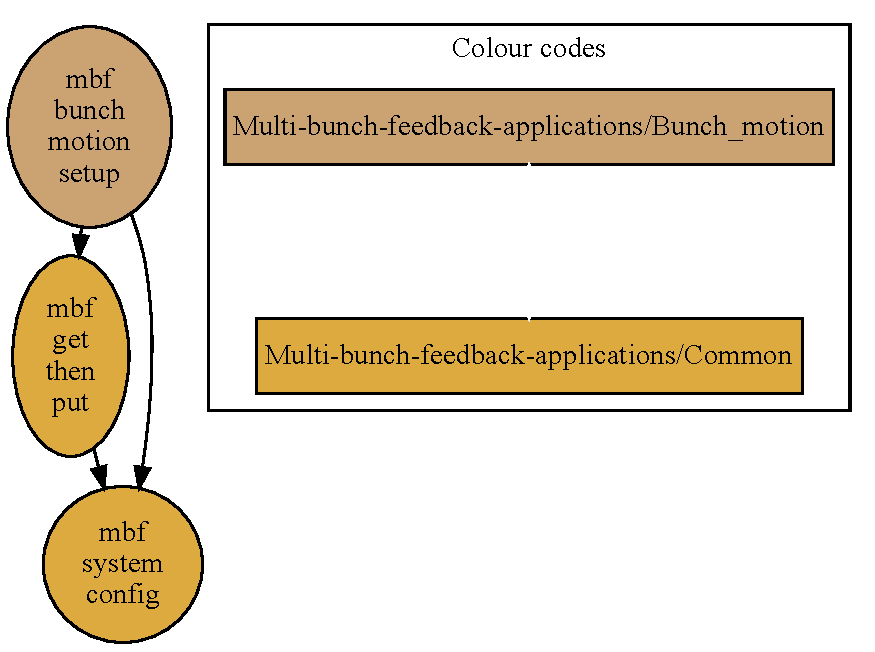
\includegraphics[width=\textwidth]{mbf_bunch_motion_setup.pdf}\\
  \caption{Code tree for bunch motion setup}\label{fig:code_tree_bunch_motion_setup}
    \end{subfigure}
       \begin{subfigure}[b]{0.6\textwidth}
  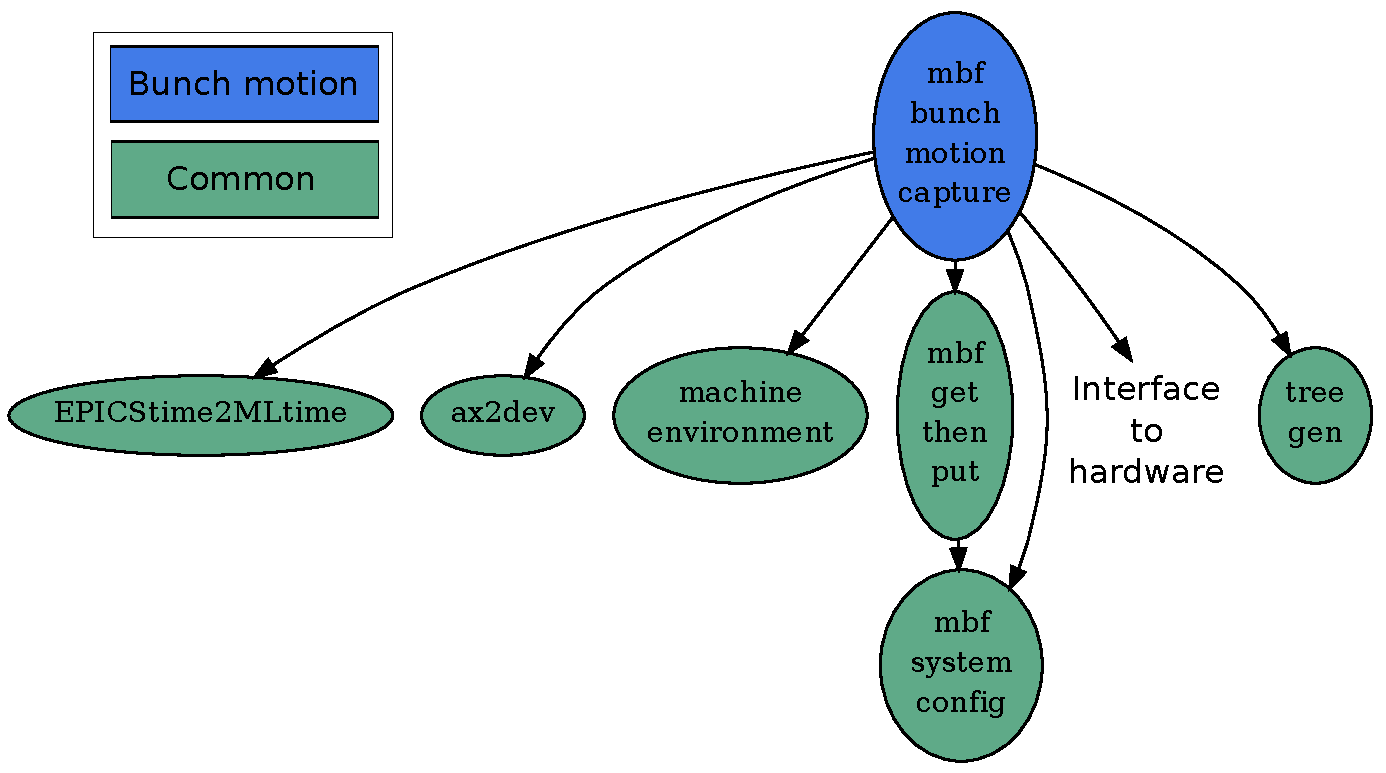
\includegraphics[width=\textwidth]{mbf_bunch_motion_capture.pdf}\\
  \caption{Code tree for bunch motion capture}\label{fig:code_tree_bunch_motion_capture}
    \end{subfigure}
    \caption{Code trees bunch motion}\label{fig:growdamp_archival_code_trees}
\end{figure}

\section{Examples}

\begin{verbatim}
mbf_bunch_motion_setup
bunch_motion = mbf_bunch_motion_capture
mbf_restore_all
mbf_bunch_motion_plotting(bunch_motion)  <--- Experimental!
\end{verbatim}

\end{document} 